%%% template.tex
%%%
%%% This LaTeX source document can be used as the basis for your technical
%%% paper or abstract. Regardless of the length of your document, the commands
%%% are all the same.
%%% 
%%% The "\documentclass" command is the first command in your file. If you want to 
%%% prepare a version of your article with line numbers - a "review" version - 
%%% include the "review" parameter:
%%%    \documentclass[review]{acmsiggraph}
%%%

\documentclass{acmsiggraph}

%%% Title of your article or abstract.

\title{Running Minion:  Jump over Obstacles using Reinforcement Learning}

\author{
  Zhaoyu Lu \\
  \texttt{zylu@ucla.edu}
  \and
  Jiayu Li \\
  \texttt{lijiayu1027@ucla.edu}
  \and
  Siyuan Qi \\
  \texttt{syqi@cs.ucla.edu}
  \and
  Yutong Zhang \\
  \texttt{yzhang@cs.ucla.edu}
  }
\pdfauthor{Stephen N. Spencer}

%%% Used by the ``review'' variation; the online ID will be printed on 
%%% every page of the content.

\TOGonlineid{45678}

% User-generated keywords.

\keywords{radiosity, global illumination, constant time}

% With the "\setcopyright" command the appropriate rights management text will be added
% to your document.

%\setcopyright{none}
%\setcopyright{acmcopyright}
%\setcopyright{acmlicensed}
\setcopyright{rightsretained}
%\setcopyright{usgov}
%\setcopyright{usgovmixed}
%\setcopyright{cagov}
%\setcopyright{cagovmixed}
%\setcopyright{rightsretained}

% The year of publication in the "\copyrightyear" command.

\copyrightyear{2016}

%%% Conference information, from the completed rights management form.
%%% The "\conferenceinfo" command has two parameters: 
%%%    - conference name
%%%    - conference date and location
%%% The "\isbn" field includes the year and month after the article ISBN.

\conferenceinfo{SIGGRAPH 2016 Posters}{July 24-28, 2016, Anaheim, CA} 
\isbn{978-1-4503-ABCD-E/16/07} 
\doi{http://doi.acm.org/10.1145/9999997.9999999}

\begin{document}

%%% This is the ``teaser'' command, which puts an figure, centered, below 
%%% the title and author information, and above the body of the content.


\maketitle

\begin{abstract}

In this project, we designed a virtural game where a Minion is running and jumping in order to survive in the harsh living environment. In the game setting, a Minion is controlled by our algorithm to run as far as possible. Along the way, the minion is running at a constant speed, and it needs to jump at an appropriate position to avoid collision with obstacles. We implemented the game in Pygame and used a reinforcement learning algorithm (Q-learning) to learn the learn a decision policy that guides the Minion to take actions at an appropriate timing. The experiments results show the superiority of our work and the learned agent could manage to survive in the cruel living environment for a long time.

\end{abstract}

%% ------------------------------------- INTRODUCTION ------------------------------------- %%
\section{Introduction}


%% ------------------------------------- RELATED WORK ------------------------------------- %%
\section{Related Work}


%% ------------------------------------- MODEL ------------------------------------- %%
\section{Model}


%% ------------------------------------- LEARNING ------------------------------------- %%
\section{Learning}


%% ------------------------------------- EXPERIMENTS ------------------------------------- %%
\section{Experiments}


\begin{figure}[ht]
  \centering
  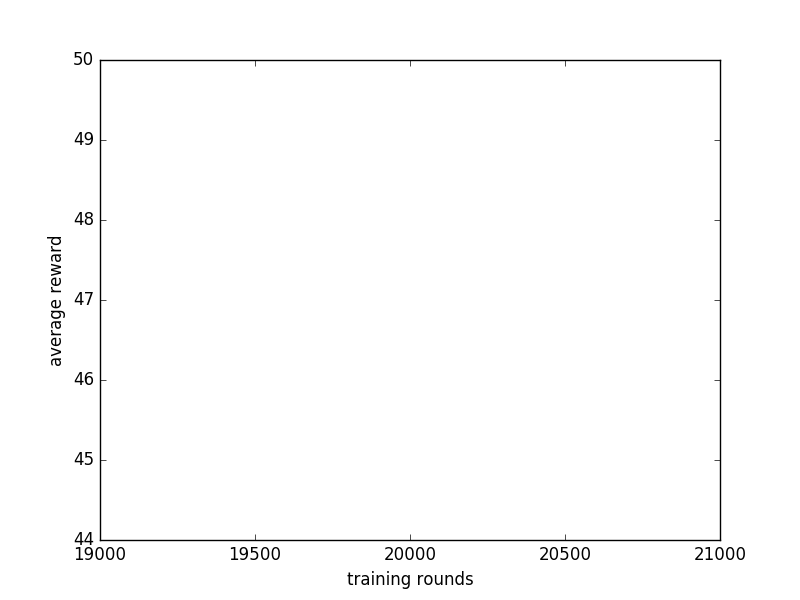
\includegraphics[width=3.0in]{../figures/testing.png}
  \caption{Testing result.''}
  \label{fig:ferrari}
\end{figure}


%% ------------------------------------- CONCLUSION ------------------------------------- %%
\section{Conclusion \& Future Work}



\section*{Acknowledgements}

To Robert, for all the bagels.

\bibliographystyle{acmsiggraph}
\nocite{*}
\bibliography{template}
\end{document}
